\chapter{We Hope You Enjoy Typing} 
\lstset{style=6502Style}
Gather round children and let me tell you about a time when kids not unlike you were
so determined to see colors on a screen that they were prepared to spend hours punching
numbers into a computer terminal with only a very slim prospect that their efforts would not be utterly 
in vain.

Prior to the release of Psychedelia in the Christmas of 1984, Jeff Minter made a cut-down version of the
software available as just such a type-in listing. This gives us a very useful specimen to work with in
explaining the mechanics of the game. 

\clearpage
\begin{figure}[H]
    \centering
    \begin{adjustbox}{width=12cm,center}
      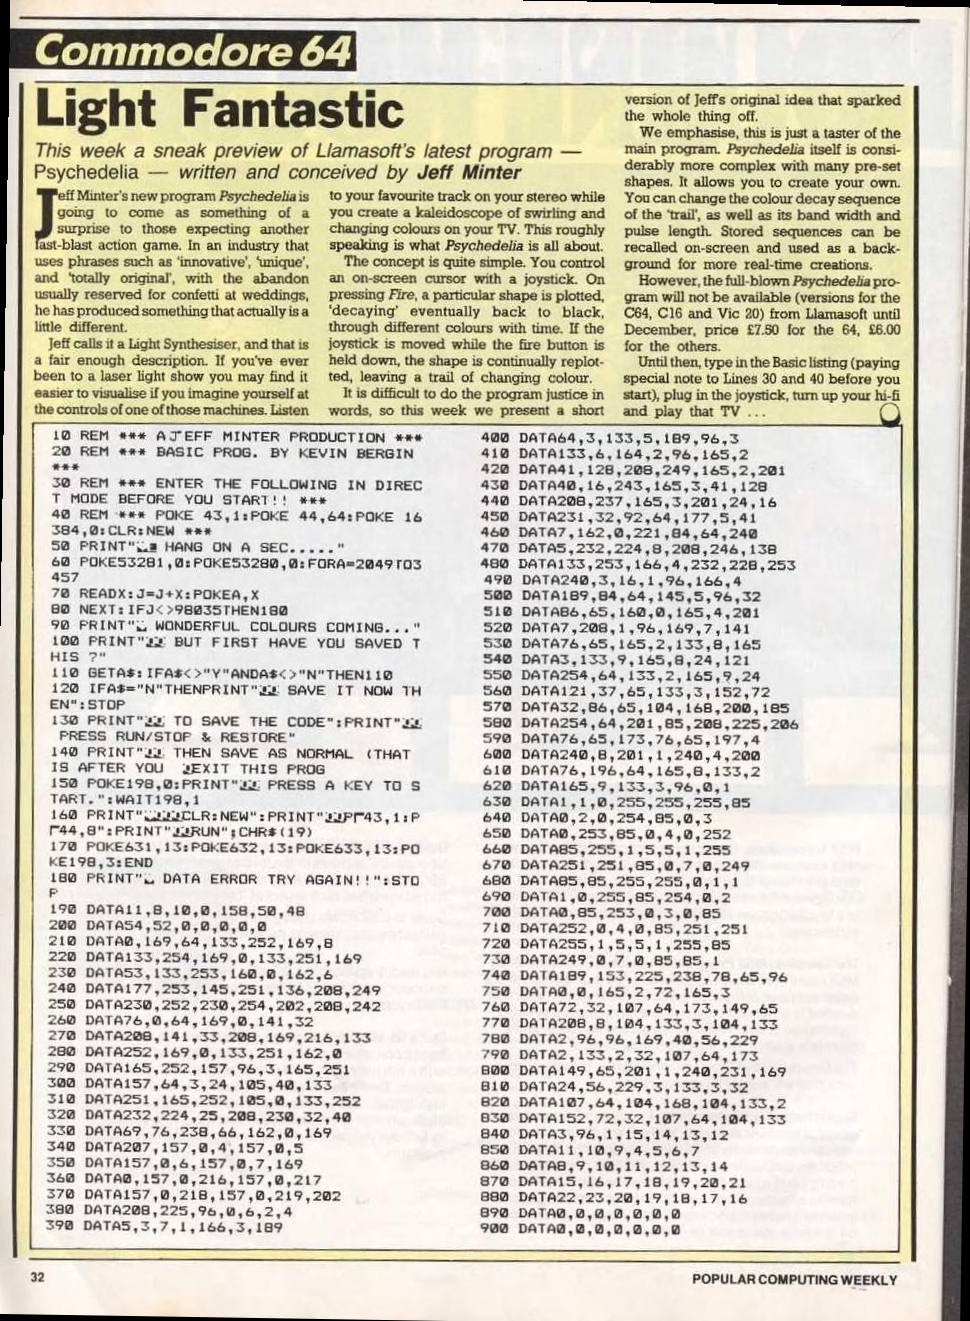
\includegraphics[width=12cm]{src/listing/PopularComputing_Weekly_Issue_1984-12-13_0031.jpg}%
    \end{adjustbox}
\caption{You are expected to type all of this. Source: Popular Computing Weekly 1984.}
\end{figure}

\begin{figure}[H]
    \centering
    \begin{adjustbox}{width=12cm,center}
      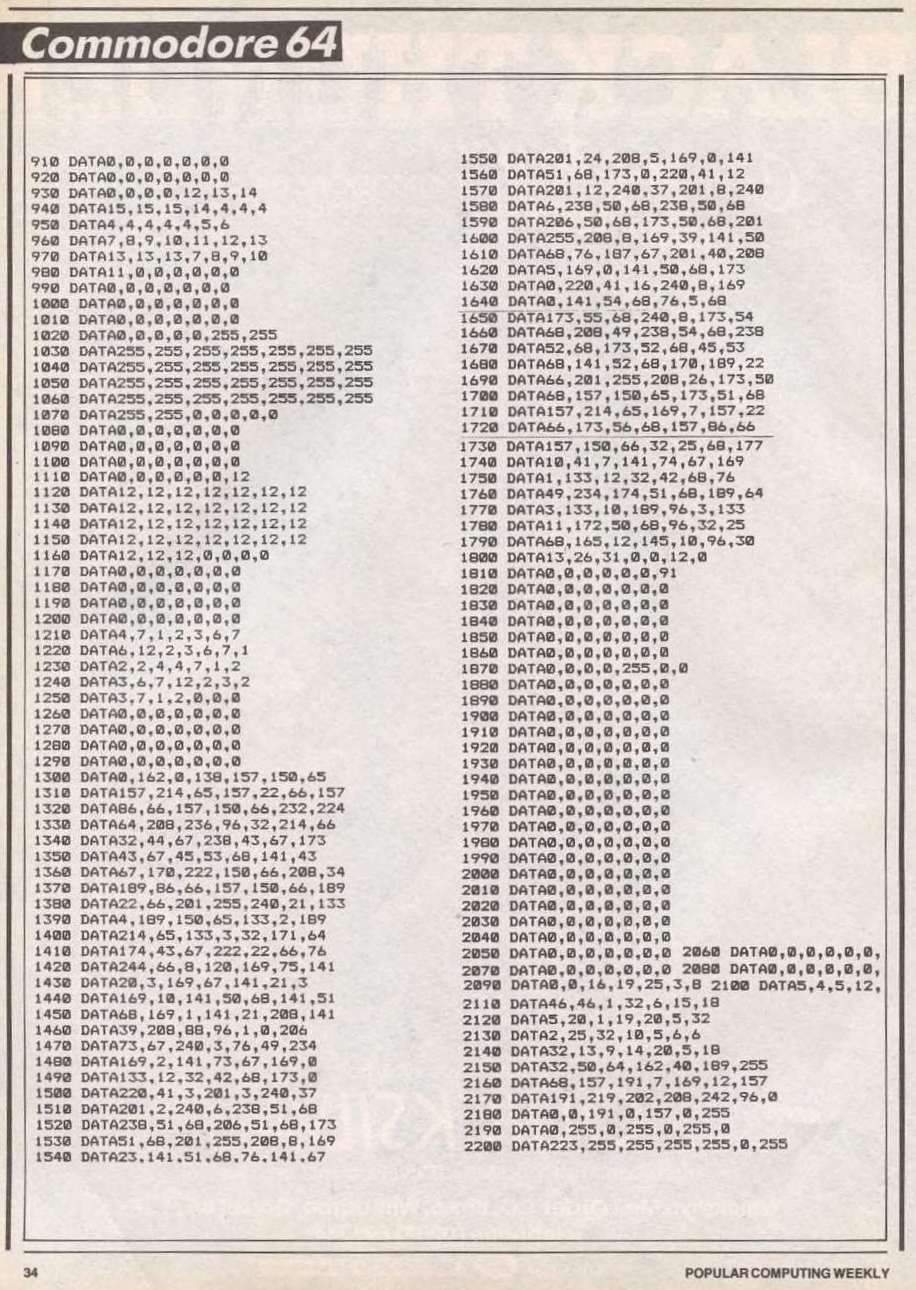
\includegraphics[width=12cm]{src/listing/PopularComputing_Weekly_Issue_1984-12-13_0033.jpg}%
    \end{adjustbox}
\caption{And this.}
\end{figure}

Like all type-in listings of its day this consisted of a small BASIC program
that loads the raw machine code into memory. The juice of the program therefore
is not in the short human-readable preamble at the start of the listing:

\lstset{style=C64BasicStyle}
\begin{lstlisting}
10  REM *** A JEFF MINTER PRODUCTION ***
20  REM *** BASIC PROG. BY KEVIN BERGIN ***
30  REM *** ENTER THE FOLLOWING IN DIREC T MODE BEFORE YOU START!! ***
40  REM *** POKE 43,1:POKE 44,44:POKE 16 384,0:CLR:NEW ***
50  PRINT "HANG ON A SEC."
60  POKE 53281 ,0:POKE 53280,0:FOR A=2049 TO 3457
70  READ X: J=J+X:POKE A,X
80  NEXT: IF J<>98035 THEN 180
90  PRINT " WONDERFUL COLOURS COMING..."
100 PRINT "&& BUT FIRST HAVE YOU SAVED THIS ?"
110 GET A$: IF A$<>"V" AND A$<>"N" THEN 110
120 IF A$="N" THEN PRINT "SAVE IT NOW THEN": STOP
130 PRINT "TO SAVE THE CODE": PRINT"PRESS RUN/STOP & RESTORE"
140 PRINT "THEN SAVE AS NORMAL (THAT IS AFTER YOU EXIT THIS PROG"
150 POKE 198,0: PRINT "PRESS A KEY TO START. " : WAIT 198,1
160 PRINT "CLR: NEW": PRINT " S2PP43, 11P (744,8":PRINT "ERUN" 3 CHRS (19)
170 POKE 631,13: POKE 632,13: POKE 633,13:POKE 198,3: END
180 PRINT "DATA ERROR TRY AGAIN!"
\end{lstlisting}

This just performs the mundane task of reading in all of the numbers in the
rest of the listing and, once done, executing those numbers as a machine code
program. Rather what we're interested in is the assembly instructions that
underlie that long list of numbers. For example:

\begin{figure}[H]
    \centering
    \begin{adjustbox}{width=12cm,center}
      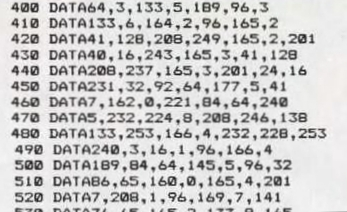
\includegraphics[width=12cm]{src/listing/PaintPixel.jpg}%
    \end{adjustbox}
\end{figure}

To give you an idea of how we get from raw numbers to an assembly program in practice I'll show you how
a little routine I call `PaintPixel` appears in the listing. Here it is:

\begin{lstlisting}
410 DATA                165,2
420 DATA 41,128,208,249,165,2,201
430 DATA 40,16,243,165,3,41,128
440 DATA 208,237,165,3,201,24,16
450 DATA 231,32,92,64,177,5,41
460 DATA 7,162,0,221,84,64,240
470 DATA 5,232,224,8,208,246,138
480 DATA 133,253,166,4,232,228,253
490 DATA 240,3,16,1,96,166,4
500 DATA 189,84,64,145,5,96   
\end{lstlisting}

If you read left to right below, you can see the decimal values given in the listing translated to
hexadecimal, then to the meaning of those hexadecimal values in 6502 assembly language.

\lstset{style=6502Style}
\begin{lstlisting}[basicstyle=\tiny]
Decimal                                   Pretty  Assembly
Data          Hex         Assembly        with labels
-------       --------    ------------    ------------------------------------------------
                                          PaintPixel                                       
165 2         A5 02       LDA $02           LDA pixelXPosition                               
41 128        29 80       AND #$80          AND #$80 ; Detect if has moved off left of screen
208 249       D0 F9       BNE $089F         BNE ReturnEarly                                  
165 2         A5 02       LDA $02           LDA pixelXPosition                               
201 40        C9 28       CMP #$28          CMP #NUM_COLS                                    
16 243        10 F3       BPL $089F         BPL ReturnEarly                                  
165 3         A5 03       LDA $03           LDA pixelYPosition                               
41 128        29 80       AND #$80          AND #$80 ; Detect if has moved off top of screen.
208 237       D0 ED       BNE $089F         BNE ReturnEarly                                  
165 3         A5 03       LDA $03           LDA pixelYPosition                               
201 24        C9 18       CMP #$18          CMP #NUM_ROWS                                    
16 231        10 E7       BPL $089F         BPL ReturnEarly                                  
32 145 8      20 91 08    JSR $0891         JSR LoadXAndYPosition                            
177 5         B1 05       LDA ($05),Y       LDA (currentLineForPixelInColorRamLoPtr),Y       
41 7          29 07       AND #$07          AND #COLOR_MAX                                   
162 0         A2 00       LDX #$00          LDX #$00                                         
                                          b408C
221 137 8     DD 89 08    CMP $0889,X       CMP presetColorValuesArray,X             
240 5         F0 05       BEQ $08CB         BEQ b4096                                        
232           E8          INX               INX                                              
224 8         E0 08       CPX #$08          CPX #COLOR_MAX + 1                               
208 246       D0 F6       BNE $08C1         BNE b408C                                        
                                          b4096   
138           8A          TXA               TXA                                      
133 253       85 FD       STA $FD           STA indexOfCurrentColor                          
166 4         A6 04       LDX $04           LDX colorIndexForCurrentPixel                    
232           E8          INX               INX                                              
228 253       E4 FD       CPX $FD           CPX indexOfCurrentColor                          
240 3         F0 03       BEQ $08D8         BEQ ActuallyPaintPixel                           
16 1          10 01       BPL $08D8         BPL ActuallyPaintPixel                           
96            60          RTS               RTS                                              
                                          ActuallyPaintPixel                               
166 4         A6 04       LDX $04           LDX colorIndexForCurrentPixel                    
189 137 8     BD 89 08    LDA $0889,X       LDA presetColorValuesArray,X                     
145 5         91 05       STA ($05),Y       STA (currentLineForPixelInColorRamLoPtr),Y       
96            60          RTS               RTS                               
\end{lstlisting}


